\documentclass[unicode]{beamer}

\usepackage[utf8]{inputenc}
\usepackage{cmap}
\usepackage[russian]{babel}

% listings
\usepackage{listings}
\lstset{language=java,frame=shadowbox,rulesepcolor=\color{gray},
        resetmargins=true,showstringspaces=false,
        basicstyle=\ttfamily,keywordstyle=\color{blue},
        stringstyle=\color{purple},commentstyle=\color{gray},
        morekeywords={assert,enum,@interface}}

% beamer
\usetheme{CambridgeUS}

\beamertemplatenavigationsymbolsempty

\setbeamertemplate{bibliography item}[book]
\setbeamertemplate{bibliography entry note}{//~}
\setbeamercolor{bibliography entry note}{fg=structure}


\title{Java-классы под капотом}
\author{Алексей Владыкин}
\date{6 ноября 2017}

\begin{document}

\begin{frame}
\titlepage
\end{frame}

\begin{frame}
\tableofcontents
\end{frame}



\section{Reflection API}

\begin{frame}
\centering

\includegraphics[width=0.6\textwidth]{pics/reflection.jpg}
\end{frame}


\begin{frame}
\begin{itemize}
\item \structure{Reflection API} --- программный интерфейс
    для получения информации об объектах и классах во время
    исполнения программы
    \bigskip

\item \texttt{java.lang.Class} и \texttt{java.lang.reflect.*}
    \bigskip

\item Для каждого типа, в том числе примитивного, можно
    получить описывающий его экземпляр класса \texttt{Class}
\end{itemize}
\end{frame}


\begin{frame}{Возможности Reflection API}
\begin{itemize}
\item Получение списка конструкторов, методов и полей класса
    \bigskip

\item Создание экземпляров класса
    \bigskip

\item Вызов методов и чтение/запись полей, в том числе закрытых
\end{itemize}
\end{frame}


\begin{frame}{Как получить \texttt{Class}}
\begin{itemize}
\item Получение класса по объекту:\\
    \lstinline|Class c1 = object.getClass();|
    \bigskip

\item Получение класса через литерал:\\
    \lstinline|Class c2 = String[].class;|\\
    \lstinline|Class c3 = int.class;|
    \bigskip

\item Загрузка класса по имени:\\
    \lstinline|Class c4 = Class.forName("java.lang.Integer");|
\end{itemize}
\end{frame}


\begin{frame}[fragile]{Как загрузить класс с диска}
\begin{lstlisting}
URL jarFileURL = 
    Paths.get("library.jar").toUri().toURL();

ClassLoader classLoader = 
    new URLClassLoader(new URL[] {jarFileURL});

Class clazz = classLoader.loadClass(
    "ru.csc.java.DemoClass");
\end{lstlisting}
\end{frame}


\begin{frame}{Имя класса}
\begin{center}
\ttfamily
\begin{tabular}{l|l|l|l}
                    & int[]     & Object[]              & Foo.Bar \\\hline
getName()           & [I        & [Ljava.lang.Object;   & Foo\$Bar \\
getCanonicalName()  & int[]     & java.lang.Object[]    & Foo.Bar \\
getSimpleName()     & int[]     & Object[]              & Bar \\
\end{tabular}
\end{center}
\end{frame}


\begin{frame}{Типы классов}
\begin{itemize}
\item \lstinline|boolean isPrimitive()|
    \bigskip

\item \lstinline|boolean isArray()|
    \bigskip

\item \lstinline|boolean isEnum()|
    \bigskip

\item \lstinline|boolean isInterface()|
    \bigskip

\item \lstinline|boolean isAnnotation()|
\end{itemize}
\end{frame}


\begin{frame}[fragile]{Специфика массивов}
\begin{lstlisting}
if (clazz.isArray()) {
    System.out.println(
            "Array of " + c.getComponentType());
}
\end{lstlisting}
\end{frame}


\begin{frame}[fragile]{Специфика enum}
\begin{lstlisting}
if (clazz.isEnum()) {
    System.out.println("Enum of:");
    for (Object e : clazz.getEnumConstants()) {
        System.out.println(e);
    }
}
\end{lstlisting}
\end{frame}


\begin{frame}{Конструкторы}
\begin{itemize}
\item Открытые конструкторы:
    \lstinline|Constructor getConstructor(Class... types)|\\
    \lstinline|Constructor[] getConstructors()|
    \bigskip

\item Все конструкторы:\\
    \lstinline|Constructor getDeclaredConstructor(Class... types)|\\
    \lstinline|Constructor[] getDeclaredConstructors()|
\end{itemize}
\end{frame}


\begin{frame}[fragile]{Вызов конструктора}
\begin{lstlisting}
Constructor constructor =
        clazz.getConstructor(String.class);

Object instance =
        constructor.newInstance("Hello World!");
\end{lstlisting}
\end{frame}


\begin{frame}{Методы}
\begin{itemize}
\item Открытые методы, в том числе унаследованные:\\
    \lstinline|Method getMethod(String name, Class... types)|\\
    \lstinline|Method[] getMethods()|
    \bigskip

\item Все методы, но только из текущего класса:\\
    \lstinline|Method getDeclaredMethod(String name, Class... types)|\\
    \lstinline|Method[] getDeclaredMethods()|
\end{itemize}
\end{frame}


\begin{frame}[fragile]{Вызов метода}
\begin{lstlisting}
Method method =
        clazz.getMethod("doSomething", int.class);

Object result =
        method.invoke(instance, 42);
\end{lstlisting}
\end{frame}


\begin{frame}{Поля}
\begin{itemize}
\item Открытые поля, в том числе унаследованные:\\
    \lstinline|Field getField(String name)|\\
    \lstinline|Field[] getFields()|
    \bigskip

\item Все поля, но только из текущего класса:\\
    \lstinline|Field getDeclaredField(String name)|\\
    \lstinline|Field[] getDeclaredFields()|
\end{itemize}
\end{frame}


\begin{frame}[fragile]{Чтение/запись поля}
\begin{lstlisting}
Field field = clazz.getDeclaredField("x");
field.setAccessible(true);

Object value = field.get(instance);

field.set(instance, null);
\end{lstlisting}
\end{frame}


\begin{frame}{Демо}
\begin{itemize}
\item JUnit
\end{itemize}
\end{frame}


\begin{frame}{Демо}
\begin{itemize}
\item Dynamic Proxy
\end{itemize}
\end{frame}



\section{Байткод Java}


\begin{frame}
\centering

\includegraphics[width=0.9\textwidth]{pics/dj_bytecode.png}
\end{frame}


\begin{frame}{Структура .class файла}
\begin{itemize}
\item Заголовок (CAFEBABE, версия формата)
\item Constant pool (числа, строки, имена классов, полей и методов)
\item Объявление класса (модификаторы, имя класса, имя суперкласса,
имена реализуемых интерфейсов)
\item Поля класса
\item Методы класса
\item Атрибуты класса (аннотации, debug info, \ldots)\\
    \texttt{javap -v -p ru.csc.java.DemoClass}
\end{itemize}
\end{frame}


\begin{frame}{Имена в байткоде}
\begin{itemize}
\item Никаких импортов, все имена полные
\item Имена классов: \texttt{java/lang/String}
\item Имена типов:
    \begin{itemize}
    \item \texttt{B, C, D, F, I, J, S, Z}
    \item \texttt{Ljava/lang/Object;}
    \item \texttt{[[I}
    \end{itemize}
\item Имена методов:
    \begin{itemize}
    \item \texttt{<init> ()V}
    \item \texttt{<clinit> ()V}
    \item \texttt{equals (Ljava/lang/Object;)Z}
    \item \texttt{toString ()Ljava/lang/String;}
    \item \texttt{sort ([III)V}
    \end{itemize}
\item Имена параметров и локальных переменных отсутствуют
\end{itemize}
\end{frame}


\begin{frame}{Исполняемый код}
\begin{itemize}
\item Состоит из простых инструкций (около 200)
\item Работает в рамках одного фрейма стека вызовов
\item Имеет локальный стек заданного размера,
    где и выполняет все вычисления
\item Может обращаться к полям и методам объектов,
    а также к своим аргументам и локальным переменным
\end{itemize}
\end{frame}


\begin{frame}{Стековая арифметика}
\begin{itemize}
\item $2+3\ \cdot\ 4$
\item $2\ 3\ 4\ \cdot\ +$
\item \texttt{iconst\_2}\\
      \texttt{iconst\_3}\\
      \texttt{iconst\_4}\\
      \texttt{imul}\\
      \texttt{iadd}
\end{itemize}
\end{frame}


\begin{frame}{Основные инструкции}
\begin{itemize}
\item Значения в стеке и локальных переменных:\\
*const*, ldc*, *load*, *store*
\item Арифметика:\\
*mul, *div, *add, *sub
\item Работа с объектами:\\
new, getfield, putfield, getstatic, putstatic
\item Вызовы методов:\\
invokestatic, invokevirtual, invokespecial, *return
\item Проверки и переходы:\\
*cmp, if*, goto*
\end{itemize}
\end{frame}


\begin{frame}
\begin{itemize}
\item Библиотека \underline{\href{http://bytebuddy.net/}{ByteBuddy}}
    \bigskip

\item Библиотека \underline{\href{http://asm.ow2.org/}{ASM}}
    \bigskip

\item Демо
\end{itemize}
\end{frame}


\begin{frame}{Практическое применение}
\begin{itemize}
\item Groovy, Kotlin, \ldots
    \bigskip
\item FindBugs
    \bigskip
\item Mockito
    \bigskip
\item Lombok
\end{itemize}
\end{frame}


\section{Расположение объекта в памяти}

\begin{frame}
\centering
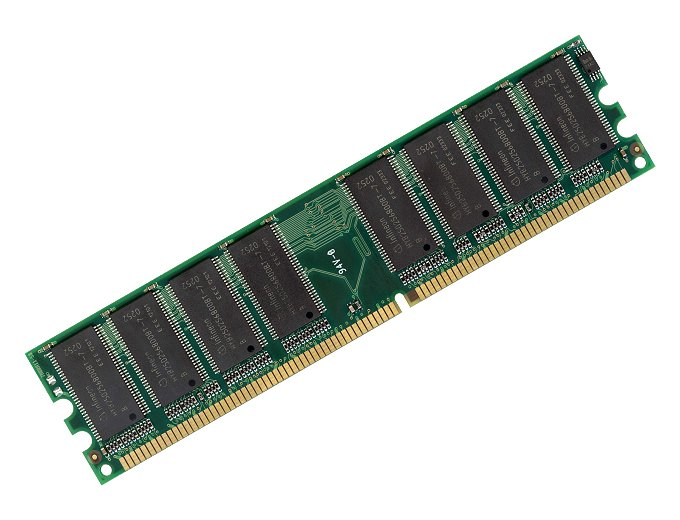
\includegraphics[width=0.8\textwidth]{pics/memory.jpg}
\end{frame}


\begin{frame}
\begin{itemize}
\item Инструмент \underline{\href{http://openjdk.java.net/projects/code-tools/jol/}{JOL}}
    \bigskip

\item Демо
\end{itemize}
\end{frame}


\end{document}
